\documentclass[letter, 11pt]{article}
\usepackage{fullpage}
\usepackage[margin=0.5in]{geometry}
\usepackage{graphicx}
\usepackage{wrapfig}
\usepackage{caption}
\usepackage{subcaption}
\usepackage{listings}
\usepackage{hyperref}
\usepackage{amsmath}
\usepackage{float}

\pagenumbering{gobble}

\begin{document}
\noindent
\large \textbf{Rahul Ghosh} \hfill \textbf{Assignment\#2}\\
\normalsize Student ID: 5476965 \hfill CSci 5561\\

\section*{SCENE RECOGNITION}
\subsection*{Methods}
\subsubsection*{Tiny Image KNN Classification}
In this method each image is resized to a small fixed resolution to get a tiny image representation. The original image and the tiny image is compared in figure 1. This tiny image is transformed to a vector and normalized to get a zero mean and unit length vector. 

Finally KNN classification is used on the vectorized data. For \textbf{k=10} the accuracy obtained is \textbf{23.8667} and the confusion matrix is shown in figure 2(a).

\subsubsection*{Bag of Word(BoW) Visual Vocabulary KNN Classification}
A Bow visual vocabulary needs to be created from the training images. For this we divide each image into 20$\times$20 cells and the residual part is ignored. Sift features are calculated for each image in those cells.  For example, if the image size is 220$\times$293, after dividing the image into 20$\times$20 and calculating the SIFT features on those, we get 140 sift features. These SIFT features are concatenated to build a pool of SIFT features from all the training images. Now we use a clustering algorithm to find the representative BoW vocabulary.

In the next step, we compute need to comoute the feature vector for each training image according to the  BoW Visual Vocabulary computed in the previous step. For this we calculate the SIFT features for each image in the same manner as in the previous step. Now given a set of SIFT features obtained from an image, the BoW features are obtained by
counting the number of SIFT features in each cluster center using nearest neighbor search.

Finally KNN classification is used on the normalized histograms. For \textbf{k=10} and \textbf{dic\_size=50} the accuracy obtained is \textbf{52.0367} and the confusion matrix is shown in figure 2(b).

Finally SVM classification is used on the normalized histograms. For \textbf{lambda=0.00005}, the accuracy obtained is \textbf{69.8667} and the confusion matrix is shown in figure 2(c).

\subsection*{Results}
\begin{figure}[H]
    \minipage{0.4\textwidth}
        \centering
        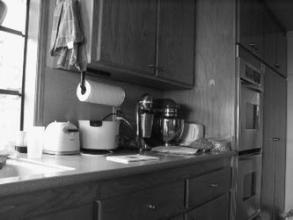
\includegraphics[width=\textwidth]{HW3/RESULT/original.png}
        \subcaption{Original Image}
    \endminipage\hfill
    \minipage{0.4\textwidth}
        \centering
        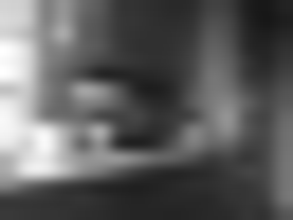
\includegraphics[width=\textwidth]{HW3/RESULT/tiny.png}
        \subcaption{Tiny Image}
    \endminipage\hfill
    \caption*{Figure 1}
\end{figure}

\begin{figure}[H]
    \minipage{0.33\textwidth}
        \centering
        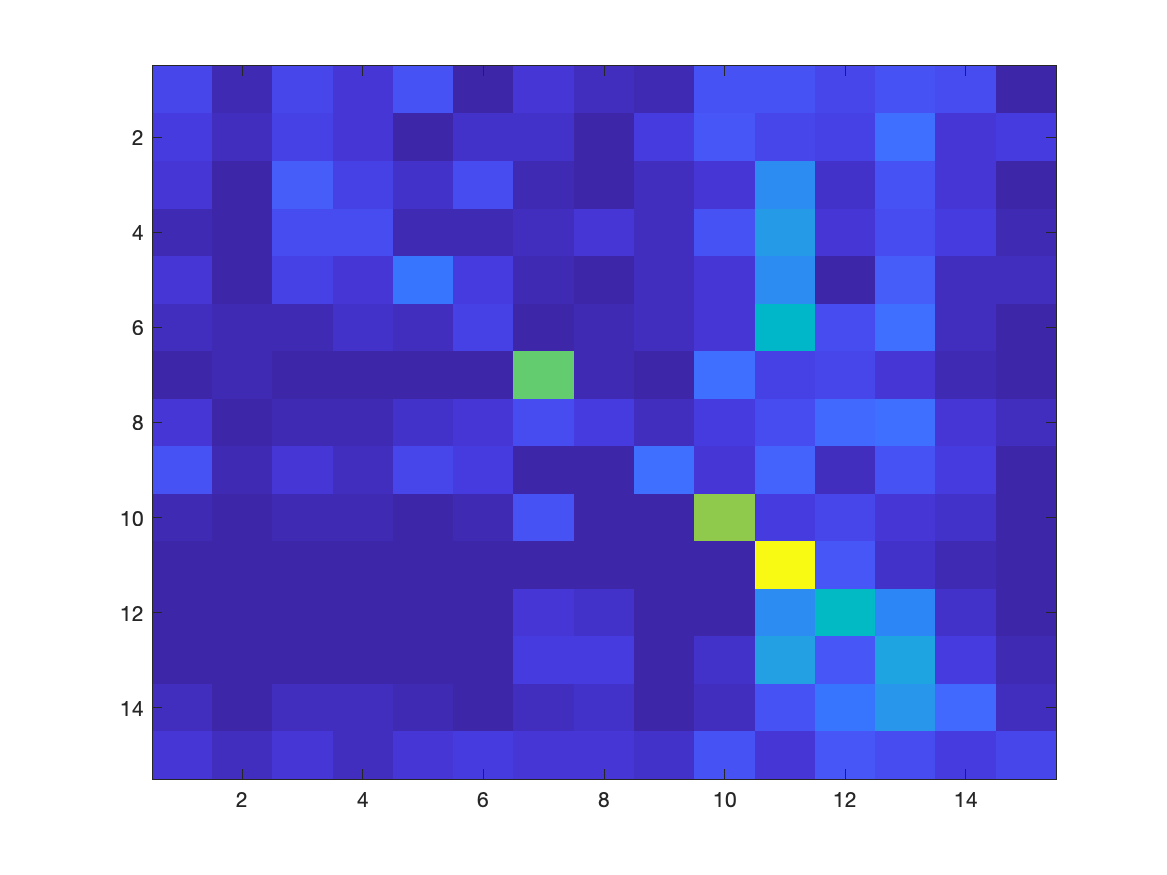
\includegraphics[width=\textwidth]{HW3/RESULT/ClassifyKNN_Tiny_confusion.png}
        \subcaption{Confusion matrix for Tiny-KNN}
    \endminipage\hfill
    \minipage{0.33\textwidth}
        \centering
        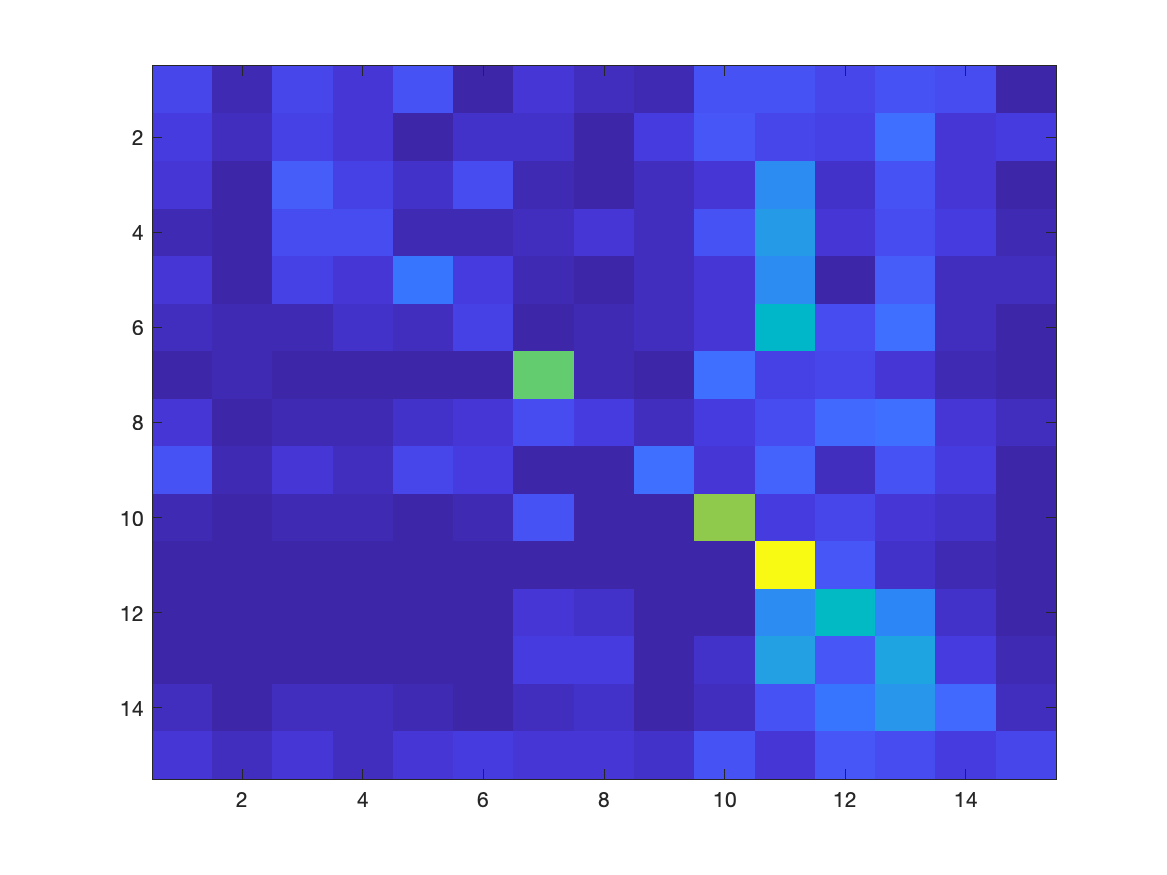
\includegraphics[width=\textwidth]{HW3/RESULT/ClassifyKNN_Tiny_confusion.png}
        \subcaption{Confusion matrix for BoW+KNN}
    \endminipage\hfill
    \minipage{0.33\textwidth}
        \centering
        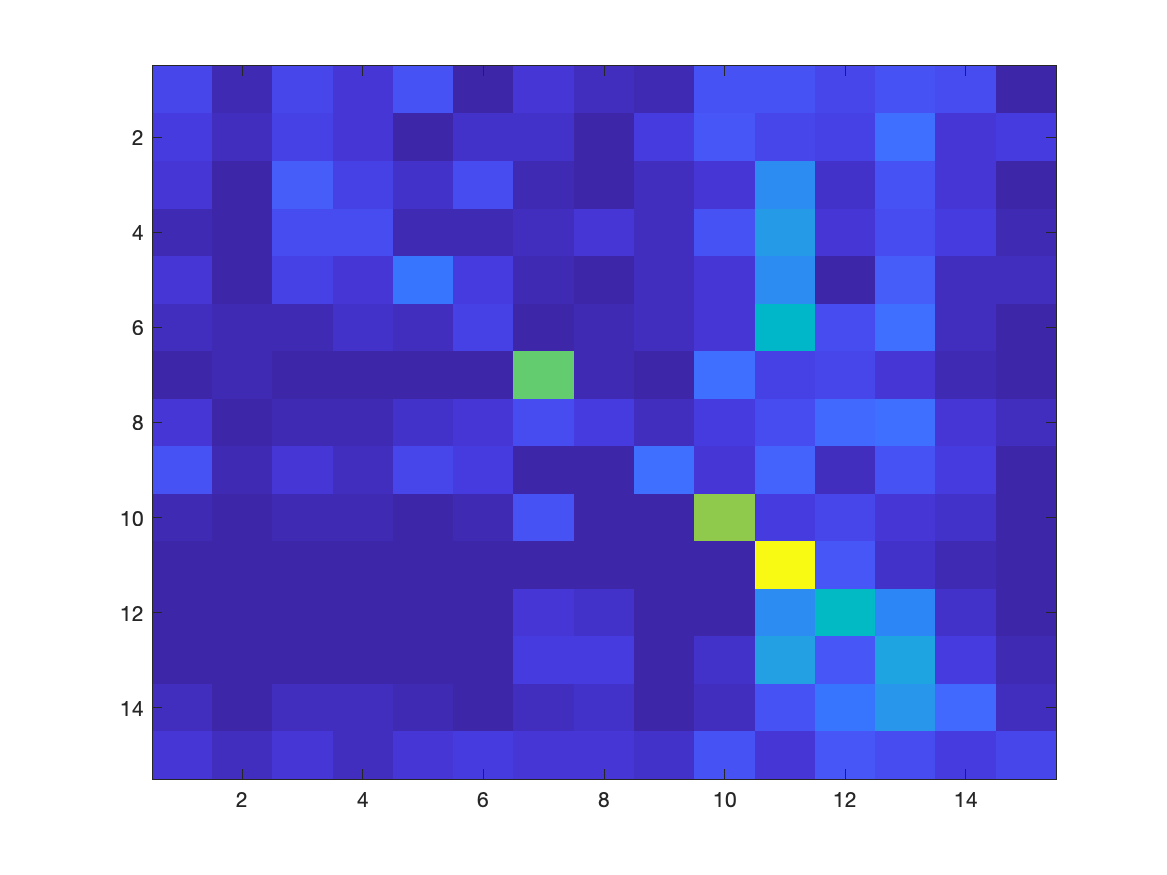
\includegraphics[width=\textwidth]{HW3/RESULT/ClassifyKNN_Tiny_confusion.png}
        \subcaption{Confusion matrix for BoW+SVM}
    \endminipage\hfill
    \caption*{Figure 2}
\end{figure}

\end{document}